\subsection{UC 20 - Eliminazione contatto} \label{sec:UC20}
    \begin{itemize}
        \item \textbf{Attore principale}: MUA;
        \item \textbf{Descrizione}: il MUA deve poter eliminare un contatto dal sistema;
        \item \textbf{Precondizioni}: l’account che il MUA gestisce è registrato nel sistema, ha una connessione aperta con il sistema ed è autenticato;
        \item \textbf{Postcondizioni}: il sistema elimina il contatto con l'identificativo fornito dal MUA;
        \item \textbf{Scenario principale}:
            \begin{enumerate}
                \item il MUA invia l'id del contatto da eliminare al sistema (\hyperref[sec:UC20.1]{UC 20.1});
                \item il sistema elimina il contatto;
            \end{enumerate}
        \item \textbf{Inclusioni}: nessuna;
        \item \textbf{Generalizzazioni}: nessuna;
        \item \textbf{Estensioni}: nessuna.
    \end{itemize}

\begin{figure}[h]
    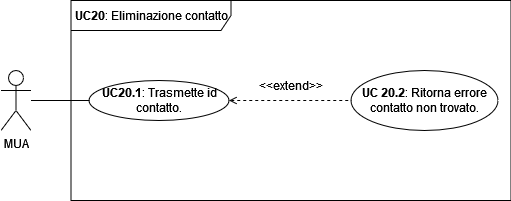
\includegraphics[width=0.85\textwidth]{sections/uc_imgs/UC20.png}
    \centering
    \caption{Diagramma sotto-casi UC 20}
\end{figure}

\subsubsection{UC 20.1 - Trasmette id contatto} \label{sec:UC20.1}
    \begin{itemize}
        \item \textbf{Attore principale}: MUA;
        \item \textbf{Descrizione}:  il MUA invia l'id del contatto da eliminare al sistema;
        \item \textbf{Precondizioni}: il MUA sta usando la funzionalità di eliminazione di un contatto;
        \item \textbf{Postcondizioni}:  il sistema conosce l'id del contatto da eliminare;
        \item \textbf{Scenario principale}:
            \begin{enumerate}
                \item il MUA invia l'identificativo del contatto da eliminare al sistema;
            \end{enumerate}
        \item \textbf{Inclusioni}: nessuna;
        \item \textbf{Generalizzazioni}: nessuna;
        \item \textbf{Estensioni}:
            \begin{enumerate}[label=\alph*.]
                \item il sistema non riesce a eliminare il contatto perché non è stato trovato:
                \begin{enumerate}[label=\arabic*.]
                    \item il sistema ritorna un errore al MUA di contatto non trovato (\hyperref[sec:UC20.2]{UC 20.2}).
                \end{enumerate}
            \end{enumerate}
    \end{itemize}


    \subsubsection{UC 20.2 - Ritorna errore contatto non trovato} \label{sec:UC20.2}
    \begin{itemize}
        \item \textbf{Attore principale}: MUA;
        \item \textbf{Descrizione}: il sistema non riesce a eliminare il contatto perché il contatto non è stato trovato;
        \item \textbf{Precondizioni}: il MUA ha inviato l'id del contatto da eliminare;
        \item \textbf{Postcondizioni}: il sistema non elimina il contatto, il MUA è stato notificato dell'errore;
        \item \textbf{Scenario principale}:
            \begin{enumerate}
                \item il sistema non trova il contatto con l'identificativo fornito dal MUA;
                \item il sistema non elimina il contatto e notifica il MUA dell'errore;
            \end{enumerate}
        \item \textbf{Inclusioni}: nessuna;
        \item \textbf{Generalizzazioni}: nessuna;
        \item \textbf{Estensioni}: nessuna.
    \end{itemize}

